\begin{figure}[h!]
    \centering
    
\includegraphics[width=0.6\linewidth]{figs/assets/pipeline.pdf}
    \caption{\textbf{An overview of the full training pipeline.} Starting with a pretrained bidirectional video diffusion model, we first finetune it with single-player and then multiplayer data. We then finetune it with a causal mask before using Self Forcing to achieve stable long-horizon autoregressive generations.}
    \label{fig:pipeline}
\end{figure}

\section{Multiplayer Training Pipeline}
\label{sec:model_architecture}
We follow the established practice of first training a bidirectional base model and then adapting it to be causal, enabling auto-regressive generation. We illustrate the stages of our training process in~\cref{fig:pipeline}.


\subsection{Stage 1: Bidirectional Single-Player}
\label{sec:bidirectional_sp_training}

We begin by initializing our model from the weights\footnote{Specifically, we use the \href{https://huggingface.co/Skywork/Matrix-Game-2.0/tree/main/base_distilled_model}{\texttt{base\_distilled\_model}} checkpoint.} of Matrix-Game 2.0~\cite{he2025matrixgame20opensourcerealtime}. \matrixgame is trained to support multiple video games in addition to Minecraft and as a result has a limited action space consisting solely of viewpoint (camera) and directional (WASD) movement. We adapt our model to support the full range of Minecraft actions by finetuning it on the VPT~\cite{baker2022videopretrainingvptlearning} dataset, which contains over 2,000 hours of human gameplay. We train the model with bidirectional attention for 120K steps with a context length of 33 frames. We find this single-player pretraining stage to be highly important as it gives our model an effective initialization for multiplayer modeling. We study this experimentally in~\cref{sec:experiments}. Throughout all stages of training, we  use the 3D VAE from \matrixgame and keep it frozen.

\subsection{Stage 2: Bidirectional Multiplayer} 

We next adapt our single-player model to support multiplayer data. We employ the architectural modifications described in~\cref{subsec:model_architecture} and train the model with full-sequence diffusion on our dataset for 120k steps, where we find that FID on a held-out test set converges at this point. This checkpoint is used as the teacher during Self Forcing (see~\cref{subsec:self-forcing} for details). 

\subsection{Stage 3: Causal Multiplayer}

To save training time, we branch training once the bidirectional model reaches 60k steps. We use this intermediate checkpoint to initialize the causal model, while the bidirectional model continues to train independently to 120k steps to serve as a high-quality teacher. Following \matrixgame, the causal model uses a sliding window attention mask with a window size of 6 latent frames (24 real frames), which serves as the maximum size of the rolling KV cache during inference. We train this model for 60k steps using diffusion forcing, and it serves as the initialization for the generator in Self Forcing. 

Our strategy of using Diffusion Forcing with a causal mask to initialize the generator is simpler than the standard CausVid~\cite{yin2025slowbidirectionalfastautoregressive} initialization of Self Forcing, which involves ODE regression and few-step distillation with DMD~\cite{yin2024one, yin2024improved} \textit{before} Self Forcing. We find our approach compares favorably to CausVid. We study this experimentally; please see~\cref{subsec:self-forcing} for details. 

\begin{figure*}[h!]
    \centering
    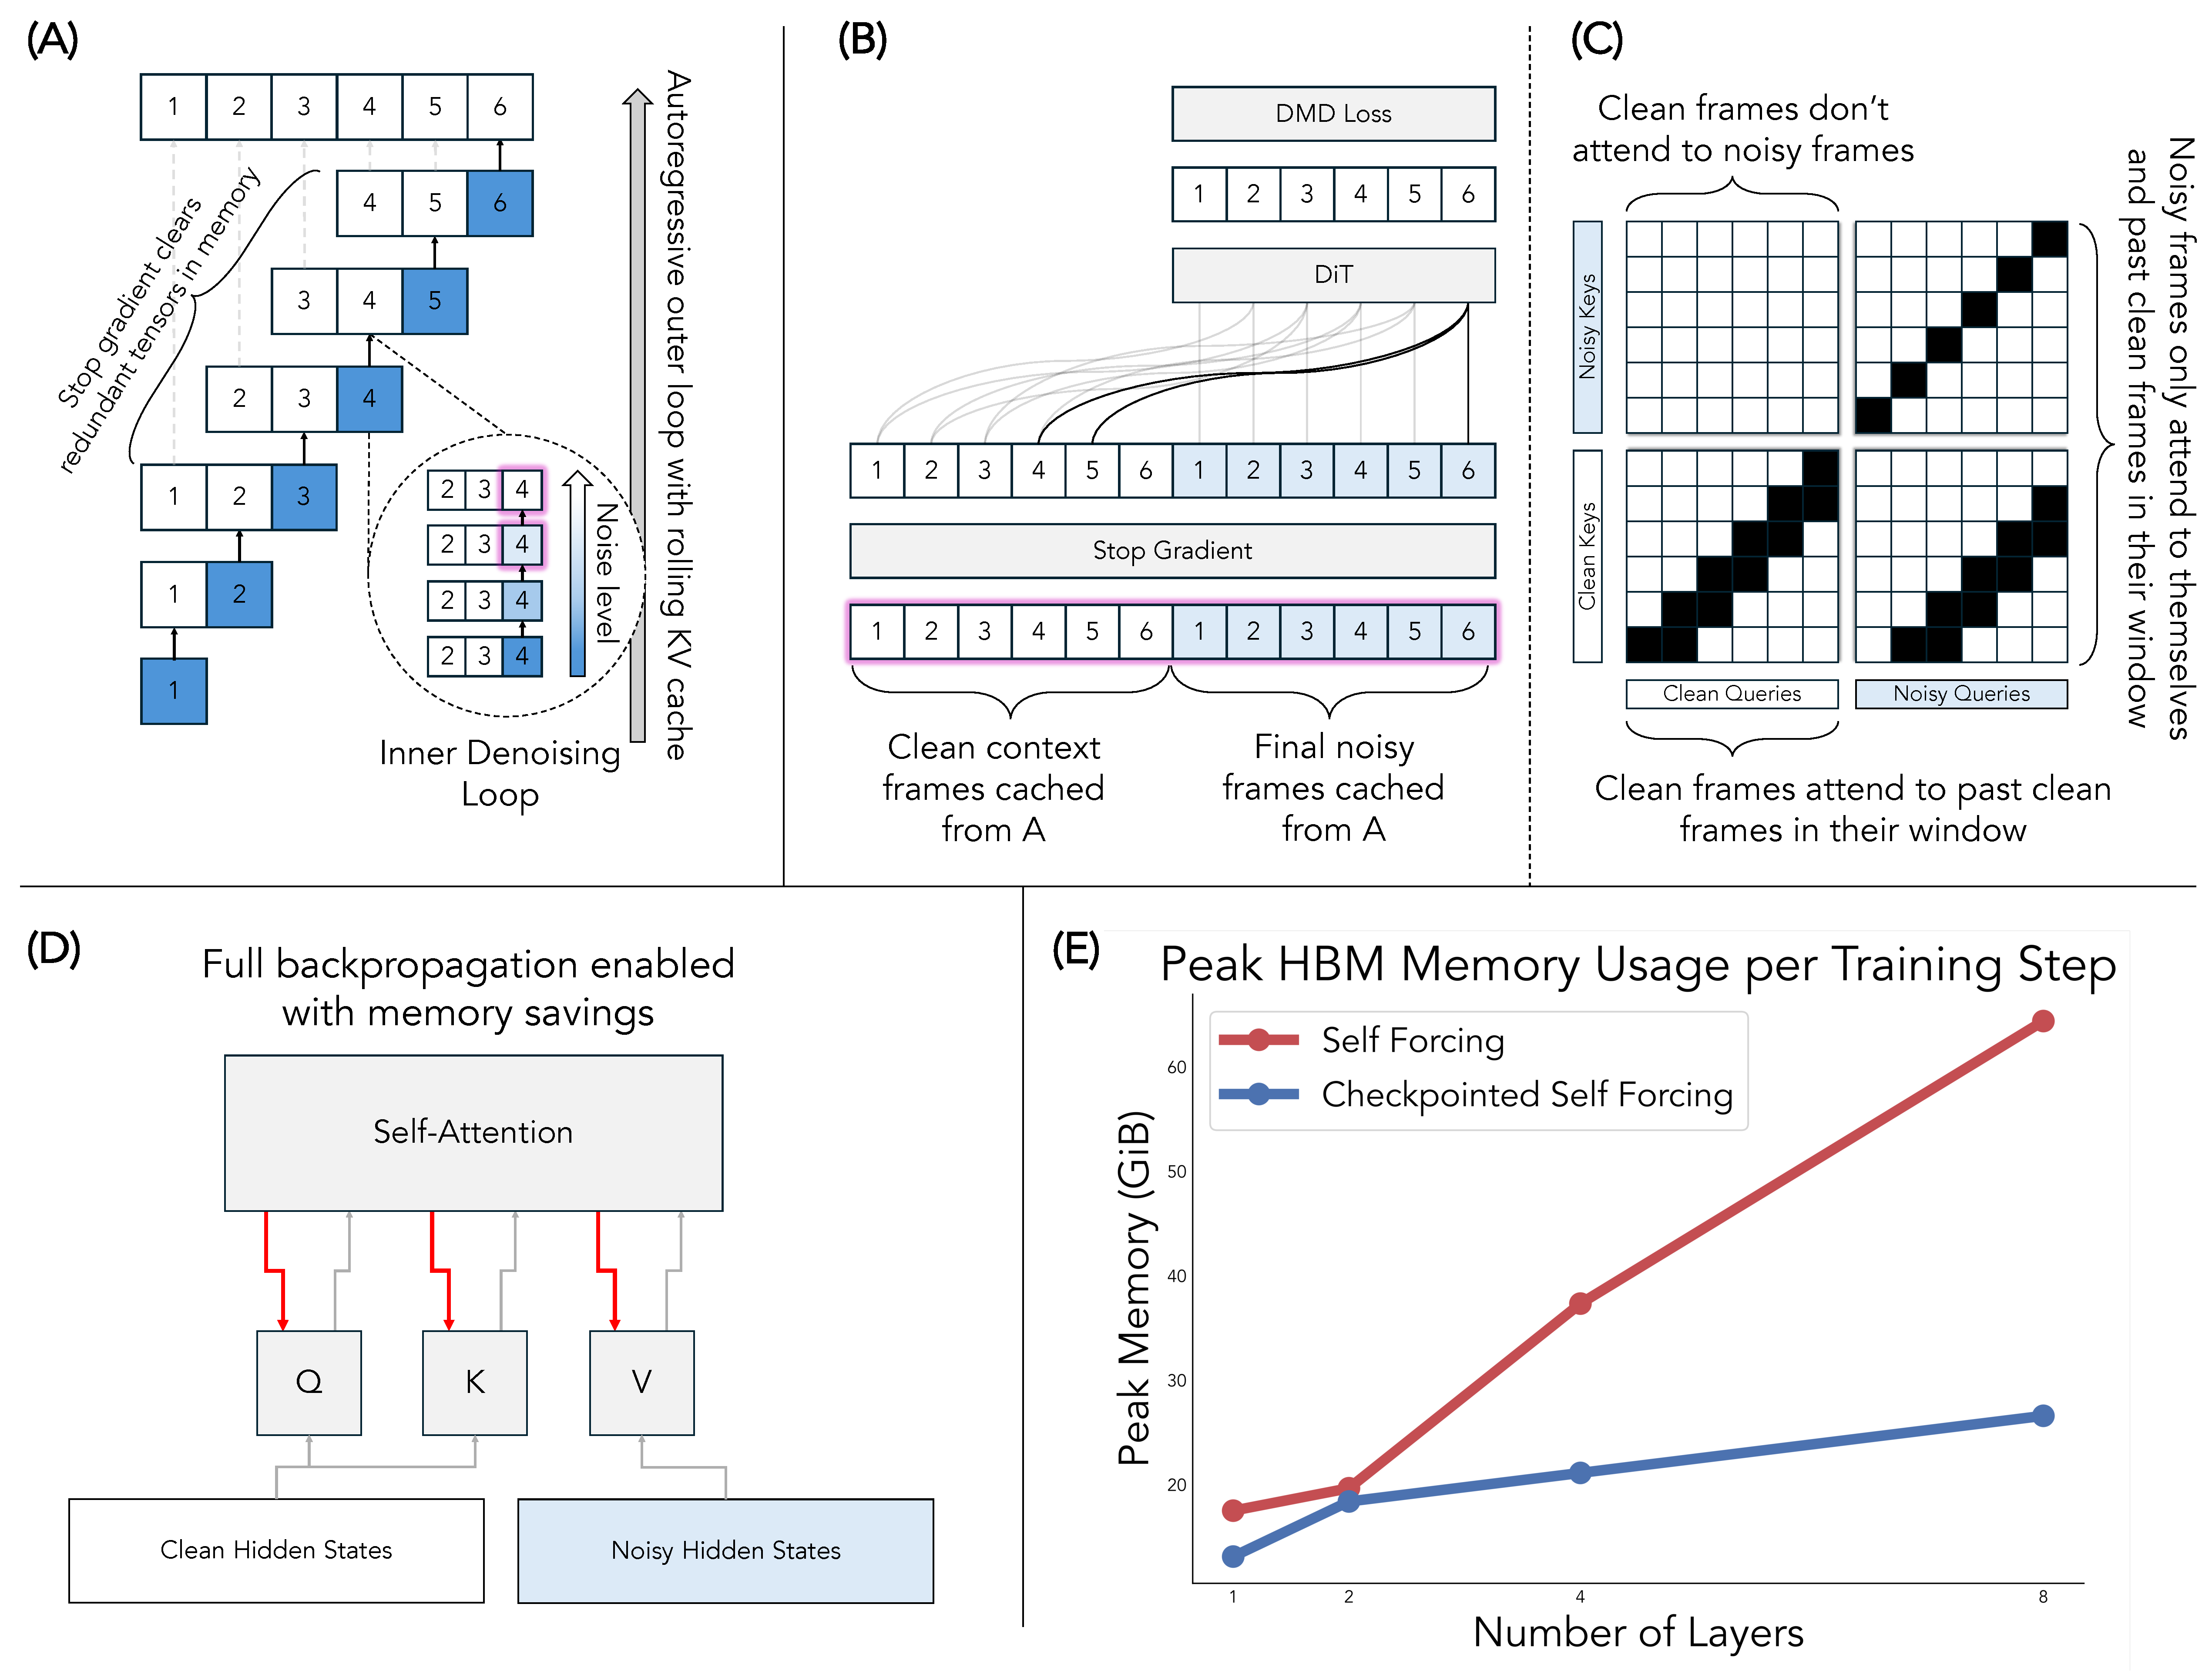
\includegraphics[width=\linewidth]{figs/assets/sf.pdf}
    \caption{An overview of \oursf. \textbf{(A)} A video is generated with a sliding-window KV cache. The computation graph in Jax contains redundant tensors, making naive backpropagation memory prohibitive. \textbf{(B)} Our recomputation step simulates the last step of denoising for every frame in parallel. Clean context frames and final noisy frames are cached from the previous step. \textbf{(C)} An illustration of the attention mask used in part B (black squares denote attention). This attention mask allows us to simulate the final denoising step of the rollout in parallel. \textbf{(D)} Leveraging these memory savings, we enable backpropagation through KV layers (avoiding the standard stop-gradient of Self Forcing), which we show improves visual generation in~\cref{sec:experiments}. Specifically, we allow gradients to flow in line 29 of~\cref{alg:self_forcing_algorithms}. \textbf{(E)} Peak memory comparison between naive and \oursf across varying depths. Scaled-down networks are used to prevent OOM errors in the naive baseline. }
    \label{fig:self_forcing}
\end{figure*}



\subsection{Stage 4: Self Forcing}
\label{subsec:self-forcing}
We apply Self Forcing~\cite{huang2025selfforcingbridgingtraintest} to improve long generations. The original Self Forcing method (see~\cref{subsec:sf_overview} for an overview) requires the context length of the student model to be equal to that of the teacher. We extend the teacher's context to be longer than the student's, allowing the student to benefit from a more powerful teacher. This requires using a sliding-window context when generating the student's video. However, naively applying Self Forcing when using this sliding window leads to excessive memory usage, as shown in~\cref{fig:self_forcing}. We fix this problem with an efficient implementation termed \textit{\oursf}. Our method first produces an initial video and caches intermediate noisy frames with gradient computation disabled. We then recompute the final video from these intermediate states in an additional step with backpropagation enabled. This process saves redundant memory that would otherwise accumulate when doing backpropagation through sliding-window video generation.

The core issue with naively applying Self Forcing in the sliding-window setting is that each generation step produces a new window of context frames, and backpropagation requires retaining all of these windows in memory simultaneously. For a student context length $L_s$ and a total generation length of $L_t$ steps, the sliding window produces overlapping windows (e.g., frames $1{:}L_s$, then $2{:}L_s{+}1$, then $3{:}L_s{+}2$), each sharing all but one frame with its predecessor. This results in a memory cost of $O(L_t \cdot L_s)$. Our method eliminates this redundancy by decoupling the autoregressive rollout from backpropagation.

Specifically, in \oursf, we first perform the autoregressive rollout to obtain the sequence of clean estimates $\hat{\mathbf{x}}_0^{1:N}$ and the corresponding noisy transition states $\mathbf{x}_{\sigma}^{1:N}$, stopping all gradient propagation during this phase. We then recompute the generator's outputs in a single parallelized forward pass. This pattern of using recomputation to save memory is analogous to Gradient Checkpointing~\cite{chen2016trainingdeepnetssublinear,griewank2000revolve}, where we manually create a checkpoint for $\hat{\mathbf{x}}_0^{1:N}$ and $\mathbf{x}_{\sigma}^{1:N}$ during the autoregressive rollout. To strictly reproduce the inference-time conditioning where noisy frames attend to clean history, we double the input sequence length by concatenating the clean frames $\hat{\mathbf{x}}_0^{1:N}$ and the noisy frames $\mathbf{x}_{\sigma'}^{1:N}$. We then apply a custom ``Teacher Forcing'' attention mask that enforces causal, sliding-window dependencies: it forces each noisy frame $\mathbf{x}_{\sigma}^i$ to attend exclusively to the preceding clean frames within its context window of size $L_s$, i.e., $\hat{\mathbf{x}}_0^{i-L_s:i-1}$. A pseudocode visualization of this procedure, which highlights the differences between \oursf and naive Self Forcing, is shown in~\cref{alg:self_forcing_algorithms}.

This formulation effectively converts the sequential rolling cache operation into a single parallel operation, reducing the memory footprint to $O(L_t)$. Due to our memory savings, we find that backpropagating through the recomputed KV representations (line 29 of~\cref{alg:self_forcing_algorithms}), though not part of the original Self Forcing algorithm, is now feasible and can improve generations (see~\cref{sec:experiments} for results).







\begin{figure}[t!]
\begin{algorithm}[H]
  \caption{\oursf}
  \small
  \SetAlgoLined
  \DontPrintSemicolon
  \KwIn{Denoise timesteps $\{t_1, \dots, t_T\}$, teacher context length $L_t$, student context length $L_s$}
  \KwIn{AR diffusion model $G_\theta$ (returns KV embeddings via $G_\theta^\text{KV}$)}

  Initialize model output $\mathbf{X}_0 \gets []$\;
  \added{Initialize noisy inputs $\mathbf{X}_s \gets []$}\;
  Initialize KV cache $\mathbf{KV} \gets []$\;
  Sample $s \sim \text{Uniform}(1, 2, \dots, T)$\;
  \For{$i \gets 1$ \KwTo $L_t$}{
    Initialize $x^i_{t_T} \sim \mathcal{N}(0, I)$\;
    \For{$j \gets T$ \KwTo $s$}{
      \If{$j = s$}{
        \added{$\mathbf{X}_s.\text{append}(x^i_{t_j})$}\;
        Set $\hat{x}^i_0 \gets G_\theta(x^i_{t_j}; t_j, \mathbf{KV})$\;
        $\mathbf{X}_0.\text{append}(\hat{x}^i_0)$\;
        \removed{Cache $\mathbf{kv}^i \gets G_\theta^\text{KV}(\texttt{stop\_grad}(\hat{x}^i_0); 0, \mathbf{KV})$}\;
        \added{Cache $\mathbf{kv}^i \gets G_\theta^\text{KV}(\hat{x}^i_0; 0, \mathbf{KV})$}\;
        $\mathbf{KV}.\text{append}(\mathbf{kv}^i)$\;
        \lIf{$|\mathbf{KV}| > L_s$}{$\mathbf{KV}.\text{pop}(0)$}
      }
      \Else{
        \removed{Set $\hat{x}^i_0 \gets \texttt{stop\_grad}(G_\theta(x^i_{t_j}; t_j, \mathbf{KV}))$}\;
        \added{Set $\hat{x}^i_0 \gets G_\theta(x^i_{t_j}; t_j, \mathbf{KV})$}\;
        Sample $\epsilon \sim \mathcal{N}(0, I)$\;
        Set $x^i_{t_{j-1}} \gets \texttt{euler\_step}(\hat{x}^i_0, \epsilon, t_{j-1})$\;
      }
    }
  }
  \added{$\mathbf{X}_s \gets \texttt{stop\_grad}(\mathbf{X}_s)$}\;
  \added{$\mathbf{X}_0 \gets \texttt{stop\_grad}(\mathbf{X}_0)$}\;
  \added{$M \gets \texttt{TeacherForcingMask}(L_s, L_t)$}\;
  \added{$\mathbf{X}_{\text{in}} \gets [\mathbf{X}_0, \mathbf{X}_s]$}\;
  \added{$\hat{\mathbf{X}}_0 \gets G_\theta(\mathbf{X}_{\text{in}}; [0, t_s], \text{mask}=M)$}\;
  Update $\theta$ via distribution matching loss\;
\label{alg:self_forcing_algorithms}
\end{algorithm}
\caption{Diff-style pseudocode comparing a single generator train step of naively applying sliding-window self forcing to our efficient implementation, \oursf. Green ``+" lines denote lines from our algorithm that have been added while red ``-" denote lines that have been removed. Please also see~\cref{subsec:teacher_forcing_mask} for mask pseudocode and~\cref{fig:self_forcing} for a visualization.}
\end{figure}

    
    



